\documentclass{article}
\usepackage[utf8]{inputenc}

\usepackage[utf8]{inputenc}
\usepackage[spanish,es-tabla,es-nodecimaldot]{babel}
\usepackage{amsmath,amsthm,amsfonts,amssymb,mathtools,dsfont,mathrsfs}
\usepackage{enumerate,graphicx,xcolor}
\usepackage{lmodern}
\usepackage[T1]{fontenc}
\usepackage[left=2cm,top=2.5cm,right=2cm,bottom=2.5cm]{geometry}
\usepackage[activate={true,nocompatibility},final,tracking=true,kerning=true,spacing=true,factor=1100,stretch=10,shrink=10]{microtype}
\usepackage{hyperref}


%\DeclarePairedDelimiter{\norm}{\lVert}{\rVert}




\newcommand{\N}{\mathbb{N}}
\newcommand{\R}{\mathbb R}
\newcommand{\Z}{\mathbb Z}
\newcommand{\Rbar}{\overline{\mathbb R}}
\newcommand{\F}{\mathscr F}
\newcommand{\A}{\mathscr A}
\newcommand{\To}{\Rightarrow}
\newcommand{\C}{\mathscr C}
\newcommand{\La}{\mathscr L_A}
\newcommand{\B}{\mathcal B}
\newcommand{\Q}{\mathbb Q}
\renewcommand{\epsilon}{\varepsilon}
\renewcommand{\L}{\mathcal L}
\renewcommand{\d}{\mathrm d}
\newcommand{\abs}[1]{\left| #1 \right|}
\newcommand{\pts}[1]{\left( #1 \right)}
\newcommand{\norm}[1]{\left\lVert#1\right\rVert}
\renewcommand{\P}[1]{\mathbb P\left( #1 \right)}
\newcommand{\E}[1]{\mathbb E \left( #1 \right)}


\newcommand{\ols}[1]{\mskip.5\thinmuskip\overline{\mskip-.5\thinmuskip {#1} \mskip-.5\thinmuskip}\mskip.5\thinmuskip} % overline short
\newcommand{\olsi}[1]{\,\overline{\!{#1}}} % overline short italic
\makeatletter
\newcommand\closure[1]{
  \tctestifnum{\count@stringtoks{#1}>1} %checks if number of chars in arg > 1 (including '\')
  {\ols{#1}} %if arg is longer than just one char, e.g. \mathbb{Q}, \mathbb{F},...
  {\olsi{#1}} %if arg is just one char, e.g. K, L,...
}
% FROM TOKCYCLE:
\long\def\count@stringtoks#1{\tc@earg\count@toks{\string#1}}
\long\def\count@toks#1{\the\numexpr-1\count@@toks#1.\tc@endcnt}
\long\def\count@@toks#1#2\tc@endcnt{+1\tc@ifempty{#2}{\relax}{\count@@toks#2\tc@endcnt}}
\def\tc@ifempty#1{\tc@testxifx{\expandafter\relax\detokenize{#1}\relax}}
\long\def\tc@earg#1#2{\expandafter#1\expandafter{#2}}
\long\def\tctestifnum#1{\tctestifcon{\ifnum#1\relax}}
\long\def\tctestifcon#1{#1\expandafter\tc@exfirst\else\expandafter\tc@exsecond\fi}
\long\def\tc@testxifx{\tc@earg\tctestifx}
\long\def\tctestifx#1{\tctestifcon{\ifx#1}}
\long\def\tc@exfirst#1#2{#1}
\long\def\tc@exsecond#1#2{#2}
\makeatother

\newtheorem{lemma}{Lema}
\newtheorem{theorem}{Teorema}

\setlength\parindent{0pt}
\setlength\parskip{4pt}


\title{Cómputo científico para probabilidad y estadística. Tarea 11.\\
Deep neural networks}
\author{Juan Esaul González Rangel}
\date{Noviembre 2023}



\begin{document}

\maketitle


\begin{enumerate}

    \item Usando la base de datos MNIST realice lo siguiente y explique cada decisión tomada:

    \begin{itemize}
        \item Diseñe una red neuronal de una sola capa oculta para la clasificación de las imágenes. Use una función de pérdida predefinida.
        


        Creando una subclase de la clase \texttt{nn.Module} de Pytorch se creó una
        red con una sóla capa oculta convolucional que toma una imagen de un canal
        y devuelve otra imagen de un canal utilizando un kernel de tamaño $4\times4$.
        Para producir la salida se aplanó el resultado de esta capa convolucional y
        se pasó por una caoa lineal (completamente conexa) y función de activación 
        \texttt{ReLu}. 

        \begin{lstlisting}[language=Python]
class NeuralNetwork(nn.Module):
    def __init__(self):
        super().__init__()
        self.conv = nn.Conv2d(1,1,4)
        self.flatten = nn.Flatten()
        self.fc = nn.Linear(25 * 25, 10)

    def forward(self, x):
        x = self.flatten(self.conv(x))
        x = F.relu(self.fc(x))
        return x \end{lstlisting}
        
        La capa convolucional sirve para extraer características de 
        las imágenes que se pasan como entradas, y como en este caso se trata de 
        números en blanco y negro, distinguir las distintas regiones dentro de la imagen
        debería ser computacionalmente sencillo, por la elección fue usar un kernel de tamaño
        $4\times4$ y con un único canal.

        Como función de pérdida se eligió la entropía cruzada y la razón es puramente
        heurística, ya que al probar con varias penalizaciones, todas arrojaban un resultado
        poco satisfactorio. De igual manera, el tipo de capa oculta que se usó en la red
        fue decidido con base en la experimentación con distintos tamaños, tipos y funciones
        de activación. Particulamente, al considerar funciones de activación que restringieran
        el rango de la salida (como sigmoide o $\tanh$), la red tendía a asignar la misma 
        etiqueta a todos los números.

        \item Entrene la red neuronal
        
        Para el entrenamiento se dividió el conjunto de datos de entrenamiento en lotes
        de 40 datos cada uno, y se iteró a lo largo de todos ellos un total de 10 épocas
        (\textit{epochs}) usando el algoritmo de descenso estocástico de gradiente con tasa
        de aprendizajde de 0.01. La elección del la tasa fue porque se trata de un valor común
        en la literatura y se recomienda comenzar con él y cambiarlo si la convergencia es muy
        lenta, como en este caso la conergencia fue adecuada, no se cambió la tasa. En cuanto
        al algoritmo de optimización, se eligió porque es un algoritmo que hemos estudiado en
        clase y tiene un fundamente teórico adecuado, además de que se recomienda su uso 
        en redes pequeñas para atacar problemas sencillos. Finalmente, la elección de la
        cantidad de épocas fue hecha para evaluar el desempeño de la red en períodos largos
        y así elegir un período de entrenamiento adecuado. Al realizar las pruebas,
        la red tiende a iniciar con un error realtiamente alto y en pocas iteraciones
        se estabiliza, luego parece oscilar en torno a un error fijo debido al carácter 
        estocástico del alrgoritmo, por lo que, aunque se entrenó la red con 10 épocas,
        se concluye que habría sido suficiente entrenarla a lo largo de 3 épocas únicamente.



        \item Presente la matriz de confusión (Confusion matrix),
        
        En la matriz de confusión se presentan como columnas los datos que la red
        predijo en cada categoría, y como filas las categorías verdaderas de los datos.
        Cada fila y cada columna están etiquetadas con una categoría, entonces si un dato
        se encuentra en la $j$-ésima columna y la $i$-ésima fila, significa que este dato
        pertenece a la $i$-ésima categoría y fue clasificado por la red dentro del tipo
        $j$. Al contar la cantidad de datos que caen en cada celda y normalizar por el
        número total de datos, obtenemos las entradas de la matriz de confusión. Evidentemente,
        una mejor matriz de confusión será más parecida a una matriz identidad, y recordemos
        que la matriz de confusión se realiza sobre el conjunto de datos de prueba (o de
        verificación, cuando está disponible). Para esta red, la matriz de confusión es 
        la siguiente,

        \begin{center}
            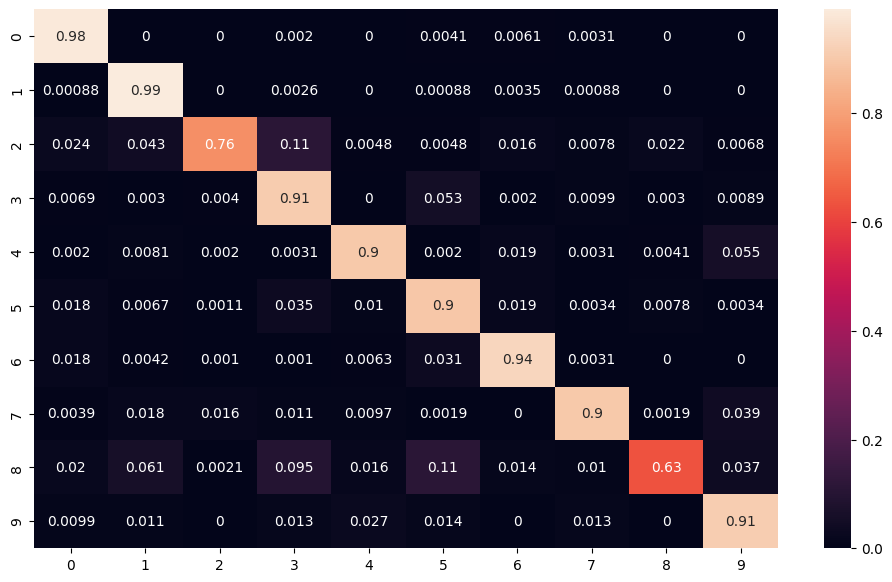
\includegraphics[width=0.9\textwidth]{./Tarea11/cm1.png}
        \end{center}

        Como podemos observar en la imagen, la mayor parte de los datos están clasificados
        de manera correcta. Particularmente el 0 y el 1 tienden a ser correctamente clasificados
        la mayor parte del tiempo, mientras que el 2 y 8 son los dígitos con los que más 
        problemas tiene la red, confundiendolos con 3 y 5.

        \item Describa que es la precisión y la exhaustividad (precision and recall) y calculelos a partir de su matriz de confusión
        
        La precisión describe qué proporción de los valores asignados por la red a una cierta clase,
        pertenecen efectiamente a esta clase. Cuanto más cercana sea la precisión, más 
        datos de los asignados a la clase en cuestión, fueron correctos. Si denotamos
        por $|\cdot|$ al cardinal de un conjunto, la precisión se puede obtener mediante,

        \begin{equation*}
            \mathrm{Precisión} = \frac{|\{\text{Datos perteneciente a la clase }j\}
            \cap \{\text{Datos asignados a la clase }j\}|}
            {|\{\text{Datos asignados a la clase } j\}|}.
        \end{equation*}

        La exhaustividad es similar a la precisión, pero en lugar de contar la cantidad de 
        datos asignados a un tipo, considera la cantidad total de datos que efectivamente
        pertenecían a este tipo, y cuenta la proporción clasificada de manera correcta.
        Usanod una notación similar a la de la precisión, la esxhaustividad se escribe como

        \begin{equation*}
            \mathrm{Precisión} = \frac{|\{\text{Datos perteneciente a la clase }j\}
            \cap \{\text{Datos asignados a la clase }j\}|}
            {|\{\text{Datos pertenecientes a la clase } j\}|}.
        \end{equation*}

        Con base en esta descripción, nos damos cuenta que para obtener la precisión de
        la categoría $j$-ésima es
        necesario dividir la entrada $j$ de la diagonal entre el total de la columna $j$,
        mientras que para obtener la exhaustividad, es necesario dividir la entrada de la 
        diagonal entre la suma de la fila. Con base en esto tenemos, para cada
        clase de este ejemplo,

        \begin{center}
            \begin{tabular}{lrrrrrrrrrr}
                \hline
                Categoría & \multicolumn{1}{l}{0} & 1 & 2 & 3 & 4 & 5 & \multicolumn{1}{l}{6} & \multicolumn{1}{l}{7} & \multicolumn{1}{l}{8} & \multicolumn{1}{l}{9} \\ \hline
                Precisión & 0.90 & 0.86 & 0.97 & 0.77 & 0.92 & 0.80 & 0.94 & 0.94 & 0.94 & 0.86 \\
                Exhaustividad & 0.98 & 0.99 & 0.76 & 0.91 & 0.90 & 0.90 & 0.94 & 0.90 & 0.63 & 0.91 \\ \hline
                \end{tabular}
        \end{center}

        Notemos que la exhaustividad corresponde exactamente a la diagonal de la matriz de
        confusión.
    \end{itemize}


    \item Usando la base de datos Fashion MNIST realice lo siguiente y explique
cada decisión tomada:

    \begin{itemize}
        \item Diseñe una red neuronal de dos capas ocultas para la clasificación 
        de las imágenes, cada una con diferente función de activación y use una 
        función de pérdida en la que el error de clasificar mal un calzado sea el 
        doble que el resto de prendas.

        Para el diseño de esta red neuronal se usaron dos capas conolucionales, la 
        primera de ella toma un canal de entrada y devuelve 20 de salida, con un
        kernel de tamaño $4\times4$, la segunda toma 20 canales de entrada y devuelve
        1 de salida usando un kernel de $3\times3$, finalmente, la capa de salida 
        toma un vector de tamaño $23\times23$ y deuelve un vector de tamaño $10\times10$.
        
        Para la primera capa se usa una función de actiación \texttt{ReLu}, mientras
        que para la segunda se usa \texttt{Elu}, que es una variante de \texttt{ReLu}
        que puede tomar valores negativos, lo que de cierta manera compensa al permitir
        disminuir la salida de una capa cuando hay varios valores positivos. 

        El código en el que se define la red es el siguiente:

\begin{lstlisting}[language=Python]
class FashionNeuralNetwork(nn.Module):
def __init__(self):
    super().__init__()
    self.conv1 = nn.Conv2d(1,20,4)
    self.conv2 = nn.Conv2d(20,1,3)
    self.flatten = nn.Flatten()
    self.fc = nn.Linear(23*23, 10)


def forward(self, x):
    x = F.relu(self.conv1(x))
    x = self.flatten(F.elu(self.conv2(x)))
    x = F.relu(self.fc(x))
    return x\end{lstlisting}
            
        Como función de pérdida se usó una variación de la entropía cruzada en la
        que se pueden agregar pesos a distintas categorías. Se ponderaron por 1 todas
        las categorías excepto \textit{Sneakers, Ankle boots} y \textit{Sandals} que
        se ponderaron por 2 para que la penalización fuera mayor al equiocarse en estos
        objetos.
        

        \item Entrene la red neuronal.
        
        Para el entrenamiento de la red neuronal se usó como optimizador \textit{Adam} que
        es una variación del descenso de gradiente estocástico, pero es adaptativo, usando
        una estimación de momentos para acelerar la convergencia. La razón para usar Adam 
        es que es un optimizador usual en redes neuronales, ya que al ser adaptativo permite
        que la convergencia sea más rápida, tanto cerca como lejos de mínimos locales.

        Al igual que en el ejercicio anterior, se dividió el conjunto de datos de entrenamientp
        en lotes de 40 datos cada uno y se entrenó a la red durante un total de 10 épocas 
        para evaluar la evolución de su rendimiento a lo largo del tiempo. De manera
        similar a como ocurrió con la red del ejercicio 1, se obtuvo que el error tendía
        a estabilizarse relativamente pronto en el entrenamiento de la red, por lo que se pudo
        haber obtenido un nivel de ajuste similar al detener el entrenamiento en 7 épocas.


        \item Presente la matriz de confusión (Confusion matrix).
        
        La matriz de confusión de la red, con un mapa de calor para visualizar el ajuste,
        es la siguiente

        \begin{center}
            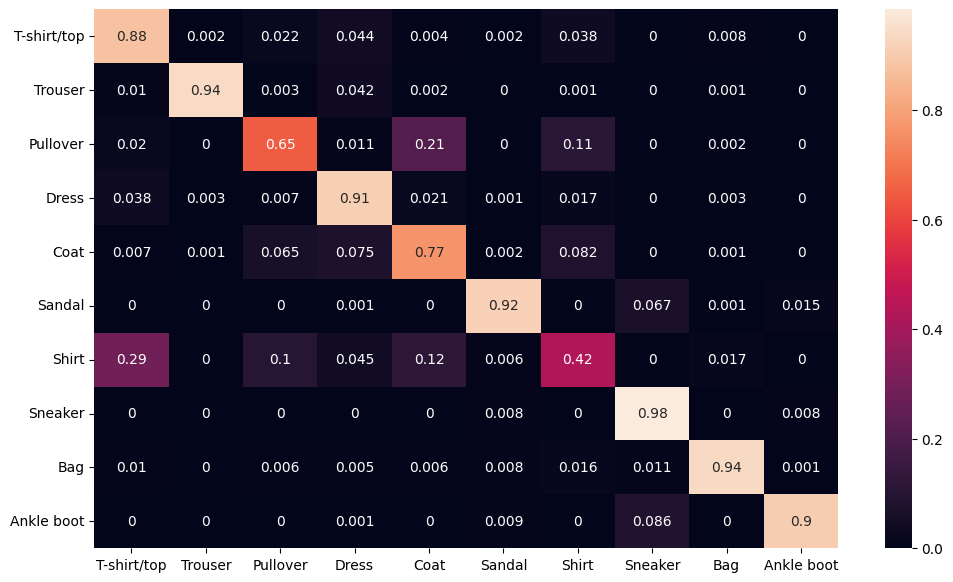
\includegraphics[width=0.9\textwidth]{./Tarea11/cm2.png}
        \end{center}

        Podemos observar que los tres tipos de clazado, junto con bolsas, vestidos y
        pantalones son los objetos que mejor reconoce la red, mientras que tiende a 
        confundir objetos como playeras con playeras de tirantes o con abrigos. Podemos
        pensar que esto es relativamente normal, pueso que una playera puede compartir 
        ciertos aspectos visuales con un abrigo, por ejemplo, y en el caso de una red sencilla
        como esta se puede complicar la extracción de características más específicas.
    \end{itemize}


    \item Con la base de datos CIFAR-10 realice lo siguiente:

    \begin{itemize}
        \item Diseñe una red neuronal de una capa oculta completamente conectada de al 
        menos 10,000 neuronas para la clasificación de las imágenes.

        El código para la implementación de esta red es el siguiente,

\begin{lstlisting}
class DenseNeuralNetwork(nn.Module):
def __init__(self):
    super().__init__()
    self.conv = nn.Conv2d(3,3,5)
    self.flatten = nn.Flatten()
    self.fc1 = nn.Linear(3*28*28, 10000)
    self.fc2 = nn.Linear(10000, 10)

def forward(self, x):
    x = F.relu(self.conv(x))
    x = self.flatten(x)
    x = F.relu(self.fc1(x))
    x = self.fc2(x)
    return x\end{lstlisting}

    La primera capa que se usa es de entrada, y es una capa convolucional que procesa
    las imágenes para extraer características de ellas, en esta capa se usa una función
    de activación \texttt{ReLu} debido a que fue la que mostró un mejor desempeño al 
    probar con varias funciones distintas. La salida de la capa de entrada es aplanada 
    a continuación para ser pasada a la capa oculta, que tiene 10,000 neuronas y usa
    de nuevo una función de activación \texttt{ReLu}. Finalmente, en la capa de salida
    se convierte de nuevo la salida de las 10,000 neuronas en un vector de tamaño 10
    que corresponde a la \textit{plausibilidad} de pertenencia a cada una de las clases.

        \item Entrene la red neuronal
        
        Para entrenar ambas redes de este ejercicio se usó la función de pérdida de
        entropía cruzada, de nuevo, con base en la experiencia de probar varias pérdidas
        y revisar con cuál se obtenía un mejor resultado. 

        El método de optimización, por su parte, se cambió en cada una de las redes, 
        para esta primera se usó \texttt{Adagrad} es es descenso de gradiente adaptativo,
        lo que significa que es una variación de descenso de gradiente que varía el
        tamaño de paso según se encuentre más cerca o más lejos de un óptimo local. La 
        razón de usar este optimizador es que al adaptar la tasa de aprendizaje de manera
        dinámica permite encontrar puntos mínimos del gradiente de manera más eficiente.

        Se entrenó la red primero durente 10 épocas, lo cuál llevó mucho tiempo, y se observó
        que el algoritmo tiende estabilizarse relativamente rápido, por lo que al final
        se trabajó únicamente con dos épocas, con las cuáles se puede obtener un nivel de 
        error similar al que se obtiene con 10.

        \item Presente la matriz de confusión (Confusion matrix).
        
        La siguiente imagen es la matriz de confusión para este modelo de red neuronal,

        \begin{center}
            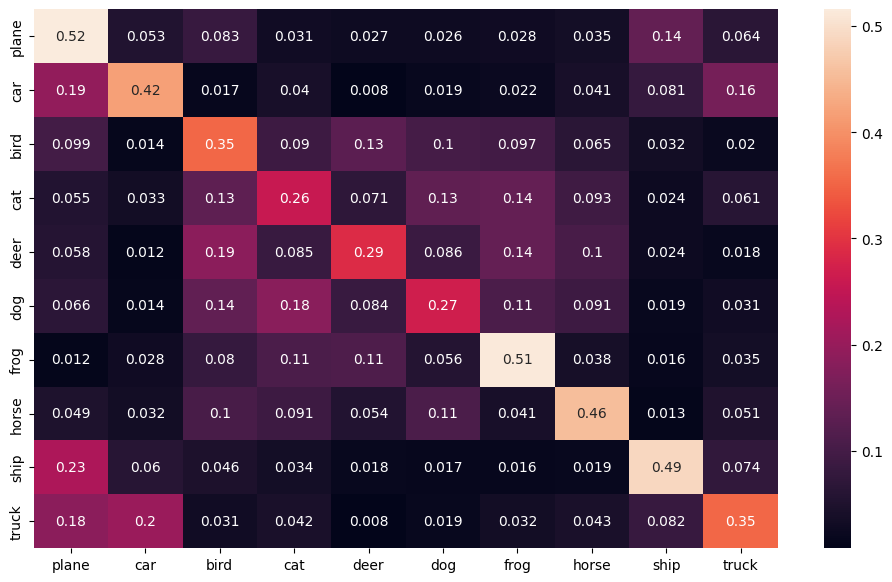
\includegraphics[width=0.9\textwidth]{./Tarea11/cm3.png}
        \end{center}

        El mejor desempeño se obtiene para ranas, caballos, barcos y aviones. Aunque
        este desempeño es mucho mejor que el trivial (10\% al elegir aleatoriamente),
        aún es algo alejado de lo que esperaríamos que hiciera un modelo competitivo de
        reconocimiento de imágenes.

        \item Entrene una segunda red neuronal usando la estructura de LeNet 5.
        
        La estructura de esta red está basada en el diagrama de LeNet5 visto durante 
        clase en la exposición del ayudante. El código de su implementación es el siguiente

\begin{lstlisting}[language=Python]
class LeNet(nn.Module):

def __init__(self):
    super(LeNet,self).__init__()
    self.conv1 = nn.Conv2d(3,6,5)
    self.pool1 = nn.MaxPool2d(2,2)
    self.conv2 = nn.Conv2d(6,16,5)
    self.fc1   = nn.Linear(16*5*5,120)
    self.fc2   = nn.Linear(120,84)
    self.fc3   = nn.Linear(84,10)

def forward(self, x):
    x = self.pool1(self.conv1(x))
    x = self.pool1(self.conv2(x))
    x = torch.flatten(x,1)
    x = F.relu(self.fc1(x))
    x = F.relu(self.fc2(x))
    x = self.fc3(x)
    return x\end{lstlisting}

    La estructura es una capa convolucionar que recibe tres canales y devuelve seis,
    a continuación es submuestrada usando el máximo en cada bloque de $2\times2$, 
    luego pasa a otra capa convolucional que convierte estos seid canales en 16
    para ser submuestreada de nuevo y luego aplanada para pasar por una capa lineal 
    con 120 neuronas, después otra lineal con 84 neuronas y finalmente una capa de
    salida que convierte esto a un vector de tamaño 10.

    En esta red se usó la misma función de pérdida que en la anterior, pero el 
    optimizador se cambió por descenso de gradiente estocástico tradicional para
    verificar su desempeño. Se entrenó la red durante 10 épocas, lo cual tuvo una
    duración de aproximadamente 1.5 horas, y se observó que el error continuaba 
    decreciendo después de varias iteraciones, aunque a un ritmo muy lento. Es posible
    que se pueda lograr un mejor ajuste de esta red, pero esto requeriría más tiempo
    y probablemente un uso más extensivo de recursos de cómputo.

        \item Presente la matriz de confusión (Confusion matrix).
        
        La siguiente es la matriz de confusión obtenida para esta estructura de red es
        la siguiente 
        \begin{center}
            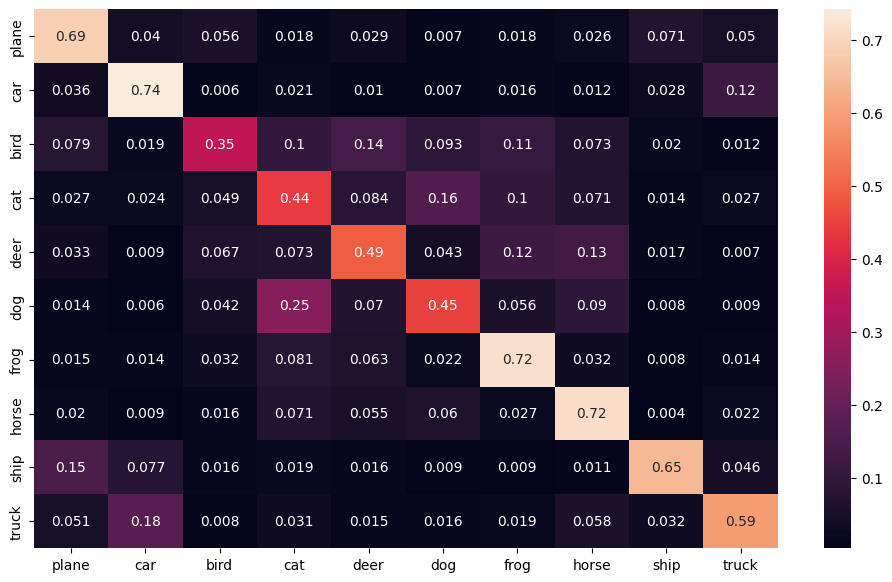
\includegraphics[width=0.9\textwidth]{./Tarea11/cm4.png}
        \end{center}

        Para esta estructura, los carros, ranas y caballos son más sencillos de identificar,
        mientras que tiene problemas identificando a los pájaros en particular y en general
        con los perros, gatos y venados, que suelen ser confundidos entre ellos.

        Los valores en la matriz de predicción de este segunod modelo son, en general,
        mejores que los valores en el modelo anterior.

        \item Compare ambas redes. Para esta comparación será necesario que al 
        menos presente las curvas de error de entrenamiento y predicción para 
        ambas redes, los tiempos de entrenamiento y que tome en cuenta las 
        matrices de confusión.

        El primer aspecto a considerar en la comparación es la complejidad computacional
        de las redes. Aunque ambas redes son muy grandes y esto causa que aumente el tiempo
        de entrenamiento, la red con las 10,000 neuronas en la capa oculta es bastante más
        pesada, al ocupar 90 mb de espacio en disco después de ser entrenada, contra únicamente
        245 kb ocupados por la red tipo LeNet5. 
        
        Como puede esperarse, el tamaño de la red repercute en su tiempo de entrenamiento,
        y el entrenamiento de 2 épocas de la red con una capa oculta llevó 3254 segundos 
        (aproximadamente 54 minutos) contra 5853 segundos (aproximadamente 97 minutos)
        que llevó entrenara LeNet5 durante 10 épocas. En la práctica es preferible usar un
        modelo que sea tanto más ligero como más rápido de entrenar.

        Además de la velocidad de entrenamiento también la podemos revisar qué tan rápido
        disminuye el error al entrenar, esto se observa en las siguientes gráficas.

        \begin{center}
        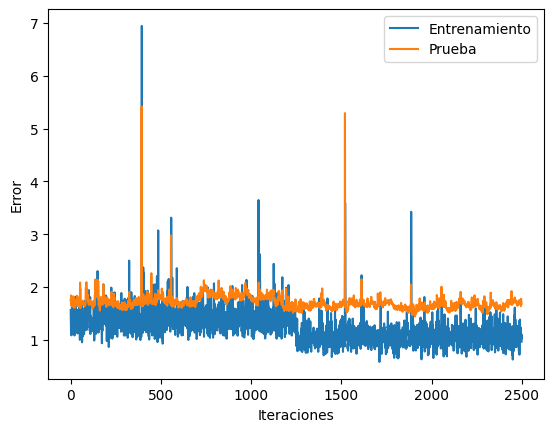
\includegraphics[width=0.55\textwidth]{./Tarea11/evo1.png}
        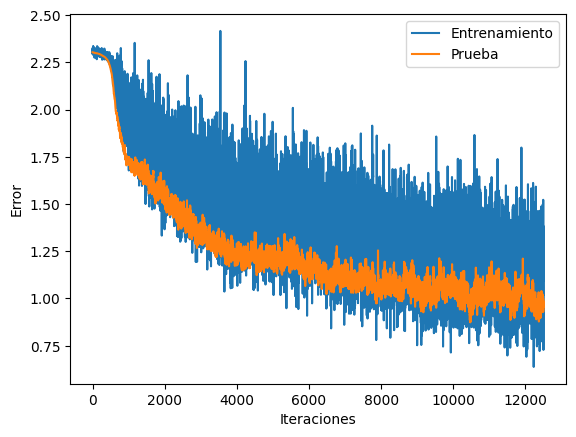
\includegraphics[width=0.55\textwidth]{./Tarea11/evo2.png}
        \end{center}

        La primera gráfica corresponde a la evolución del error a lo largo del entrenamiento
        de la red con 10,000 neuronas en una capa oculta. Podemos ver que el error de prueba
        se mantiene aproximadamente constante a lo largo del entrenamiento, mientras que 
        el error de entrenamiento disminuye de manera muy lenta. Esto parece sugerir
        que la red se está sobreajustando, pero aún este sobreajuste ocurre muy lentamente,
        por lo que pareciera que para esta estructura en particular es complicado
        trabajar con los datos de CIFAR10.

        En la segunda gráfica, que corresponde a la red con estructura de LeNet5, se 
        observa que tanto el error de entrenamiento como el de prueba disminuyen a 
        medida que se entrena más, aunque ambos parecen estabilizarse eventualmente.
        
        Notemos que en ambas gráficas el error no es una fucnión monótona y presenta 
        ruido, pero esto se debe a que debido a las características estocásticas del
        algoritmo, en algunas ocasiones se avanza en dirección subóptima, sin embargo,
        después de varias iteraciones, se espera que disminuya el error eventualmente.

        Un tercer criterio de ecisión entre los modelos es las matrices de confusión.
        Podemos notar que con un tiempo de entrenamiento similar, el desempeño de la red
        LeNet5 es bastante superior al de la red con 10,000 neuronas en una capa.

        Con base en los puntos anteriores, es posible afirmar que la arquitectura de
        LeNet5 es superior a la de una capa con 10,000 neuronas para la clasificación
        del conjunto de datos CIFAR10. La conclusión de esta comparación es que el poder
        de las redes neuronales no se basa únicamente en su flexibilidad al contar con
        un gran número de parámetros que ajustar, sino en que la configuración que tienen
        como composición de funciones logra aproximaciones más eficientes.

    \end{itemize}


    El código de esta tarea puede encontrarse en este url \url{https://colab.research.google.com/drive/1ASPPkaoMB3N1NqnDmU_eo0yz7u5cZkeX?usp=sharing}

    % \item Usando la base de datos MNIST y la estructura LeNet 5 realice lo siguiente:

    % \begin{itemize}
    %     \item Entrene la red neuronal
    %     \item Implemente el algoritmo \textit{Deepfool} y construya un ejemplo adversario para cada una de las categorías, presente la imagen original, el ruido que añadió y la nueva imagen. 
    % \end{itemize}

    % Hacer el conjunto de entrenamiento, prueba y evaluación
        
   
\end{enumerate}




 \end{document}